

\begin{document}
	\begin{titlepage}
		\begin{center}
		
			\begin{minipage}{4.5cm}
				\begin{center}
					
\includegraphics[width=5cm,height=4cm]{ehtp.png}
				\end{center}
			\end{minipage}
			
			\textsc{\Large }\\[1.5cm]
			{\large \bfseries Rapport de Projet}\\[0.5cm]
			{\large Réseau}\\[1cm]
			
			{\large \bfseries Filière : Génie Informatique}\\[1cm]
			
			\rule{\linewidth}{0.3mm} \\[0.4cm]
			{ \huge \bfseries\color{blue!70!black}DNS, HTTPS,LDAP, FTP, SMTP, IMAP \\[0.4cm] }
			\rule{\linewidth}{0.3mm} \\[1cm]
			
			\noindent
			\begin{minipage}{0.4\textwidth}
				\begin{flushleft} \large
					\emph{\color{orange!80!black}Réalisé par :}\\
					Yassine \textsc{Noureddine}\\
					Slimani \textsc{Mohamed Amine}\\
					Assadiki \textsc{ Zaid}\\
				\end{flushleft}
			\end{minipage}%
			\begin{minipage}{0.5\textwidth}
				\begin{flushright} \large
					\emph{\color{orange!80!black}Encadré par :} \\
					Rghioui \textsc{Anass}
				\end{flushright}
			\end{minipage}\\[1cm]
			
			\vfill
			
			{\large \color{orange!80!black}{Année universitaire}\\ \color{blue!80!black}2024/2025}
			
		\end{center}
	\end{titlepage}
	
	\newpage
	
	\renewcommand{\thesection}{\Roman{section}}  % Sections en chiffres romains majuscules
		\section{Introduction}
Dans le paysage en constante évolution de l'informatique et des technologies de l'information, la configuration adéquate des protocoles réseau est un élément crucial pour assurer la connectivité, la sécurité et le bon fonctionnement des systèmes. Avec l'essor des technologies numériques, la demande en infrastructures réseau fiables et performantes s'intensifie. C'est dans ce contexte que notre projet s'inscrit, visant à mettre en œuvre une configuration robuste des principaux protocoles réseau tels que DNS, HTTPS, FTP, SMTP, IMAP, ainsi qu’un annuaire centralisé via LDAP, pour répondre aux exigences croissantes en termes de communication, de gestion des utilisateurs et de protection des données.

Le Domain Name System (DNS) joue un rôle fondamental en permettant la traduction des noms de domaine en adresses IP, rendant les sites web accessibles aux utilisateurs finaux de manière transparente et rapide. Une configuration optimisée du DNS garantit une résolution de nom fluide tout en protégeant contre des attaques telles que l’empoisonnement de cache ou le détournement de requêtes.

Le protocole HTTPS, devenu un standard incontournable, assure une communication sécurisée via le chiffrement des données échangées entre les clients et les serveurs web. Ce protocole est essentiel pour protéger les informations sensibles, comme les identifiants ou les transactions financières, et pour établir la confiance des utilisateurs en leur garantissant une navigation sécurisée.

Les protocoles de transfert et de gestion des données, tels que FTP, SMTP, et IMAP, occupent des fonctions spécifiques mais tout aussi importantes. FTP permet un échange efficace de fichiers entre systèmes, essentiel pour la gestion documentaire ou la synchronisation des données. SMTP (Simple Mail Transfer Protocol) est le moteur de l’envoi de courriels, tandis que IMAP (Internet Message Access Protocol) offre un accès flexible aux boîtes de messagerie, permettant une consultation en temps réel des courriels sur divers dispositifs.

En complément, LDAP (Lightweight Directory Access Protocol) joue un rôle central dans la gestion des identités et des accès au sein des systèmes réseau. Ce protocole permet de centraliser les informations sur les utilisateurs, les groupes, et les ressources, simplifiant ainsi l'administration tout en renforçant la sécurité. En intégrant OpenLDAP dans notre projet, nous avons mis en place un service d'annuaire qui garantit une gestion unifiée et efficace des données tout en facilitant l'accès sécurisé aux ressources réseau.

Cependant, la mise en œuvre de ces protocoles n’est pas sans défis. Les aspects techniques tels que la compatibilité des systèmes, les performances, ou encore la mise en place de mesures de sécurité avancées comme l’authentification multi-facteurs, représentent des étapes complexes mais nécessaires. En outre, des considérations telles que la protection contre les attaques de type déni de service (DDoS), le chiffrement des communications et la gestion des certificats numériques viennent compléter les enjeux de configuration.

Ce rapport détaille les étapes de notre projet, incluant une analyse approfondie des besoins, une planification rigoureuse des configurations, et la mise en œuvre de solutions adaptées. Les méthodologies suivies, combinées à une veille technologique constante, ont permis d’identifier et de résoudre les difficultés rencontrées, tout en optimisant les performances des protocoles.

En examinant minutieusement ces composants essentiels, nous visons à renforcer la résilience, la performance et la sécurité de notre infrastructure réseau, offrant ainsi une base solide pour soutenir les opérations actuelles.
	\newpage
	\tableofcontents
	\newpage
	\listoffigures
	
	\newpage
	
	\section{Configuration d'un Serveur DNS avec BIND}
	
	Le DNS (\textit{Domain Name System}) convertit les noms de domaine en adresses IP. Apache utilise ensuite ces informations pour déterminer quel site doit être servi et renvoyer la page correspondante. Cela permet d’établir une communication fluide et rapide entre les utilisateurs et les serveurs web.
	
	Dans ce projet, nous allons configurer un serveur DNS. Le logiciel utilisé est \textbf{BIND} (\textit{Berkeley Internet Name Domain}), qui est l’un des serveurs DNS les plus populaires. L’adresse IP de la machine configurée est : \textbf{192.168.245.49}.
	
	\subsection*{Configuration et Vérification}
	
	Toutes les commandes nécessaires seront exécutées en tant qu’administrateur afin d’avoir les permissions requises. Une fois BIND installé et configuré, il est important de vérifier que le service fonctionne correctement.
	
	Pour vérifier l'état du service \texttt{bind9}, nous utilisons la commande suivante :
	
	\begin{lstlisting}[language=bash]
	sudo systemctl status bind9
	\end{lstlisting}
	
	Cette commande permet d’afficher l’état du service. Si le service est actif, vous verrez une sortie similaire à celle-ci :
	
	\begin{lstlisting}[language=bash]
	service bind9 status
	\end{lstlisting}
	
	\begin{figure}[h]
		\centering
		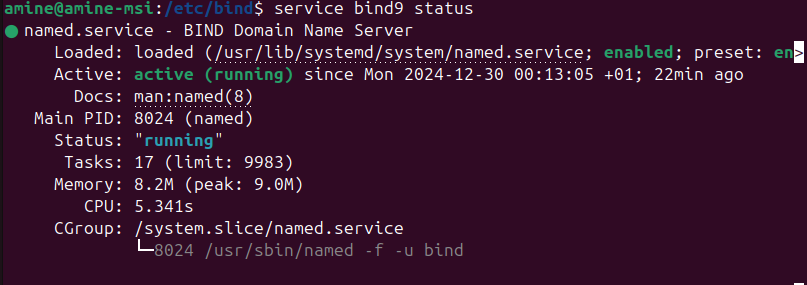
\includegraphics[width=0.7\textwidth]{DNS/status_bind9.png}
		\caption{le service est actif}
		\label{fig:ridal}
	\end{figure}

	Le service \texttt{bind9} est en activité et fonctionne correctement.

	\subsection*{Configuration des fichiers de zone}
	
	Le nom de ma machine est : DNSserver. Le nom de domaine est : \texttt{groupe7.ehtp}. Le FQDN (Fully Qualified Domain Name) est : \texttt{Dnsserver.groupe7.ehtp}.

	Les fichiers utilisés pour la configuration sont :
	\begin{itemize}
		\item \texttt{named.conf} : Configuration principale du serveur BIND.
		\item \texttt{named.conf.default-zones} : Configuration des zones par défaut.
		\item \texttt{db.local} : Fichier de configuration des enregistrements DNS pour une zone spécifique.
	\end{itemize}
	
	\subsubsection*{Création des fichiers de zone}
	
	Nous avons créé deux fichiers supplémentaires dans le dossier \texttt{/etc/bind} : \texttt{db.zonedirect} et \texttt{db.zoneinverse}.
	
	Le fichier \texttt{db.direct} contient les enregistrements DNS pour la résolution directe (nom de domaine vers adresse IP). Voici la configuration de ce fichier :
	
	\begin{figure}[h]
		\centering
		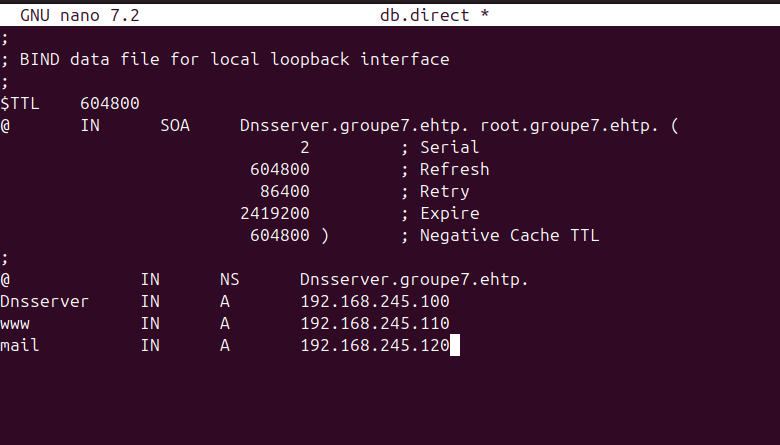
\includegraphics[width=0.7\textwidth]{DNS/db-direct.png}
		\caption{Configuration du fichier \texttt{db.direct}}
		\label{fig:ridal}
	\end{figure}

	Le fichier \texttt{db.inverse} permet de configurer la résolution inverse (adresse IP vers nom de domaine). Voici la configuration de ce fichier :
	
	\begin{figure}[h]
		\centering
		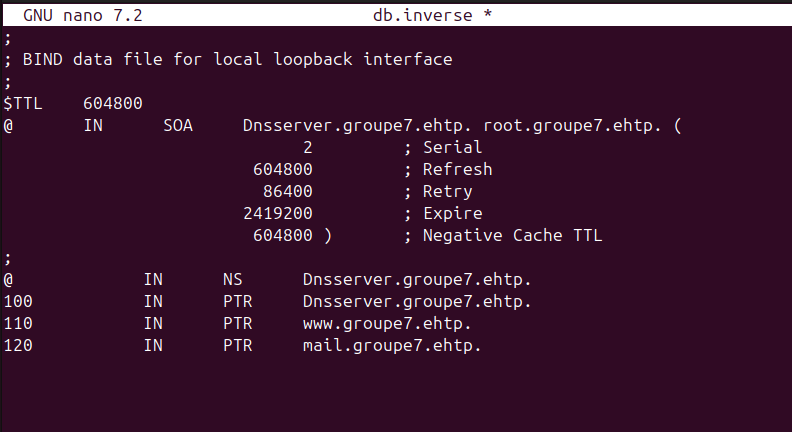
\includegraphics[width=0.7\textwidth]{DNS/db-inverse.png}
		\caption{Configuration du fichier \texttt{db.inverse}}
		\label{fig:ridal}
	\end{figure}
	
	Ensuite, nous avons modifié le fichier \texttt{named.conf.local} pour configurer les zones, comme suit :
		\newpage
	\begin{figure}[h]
		\centering
		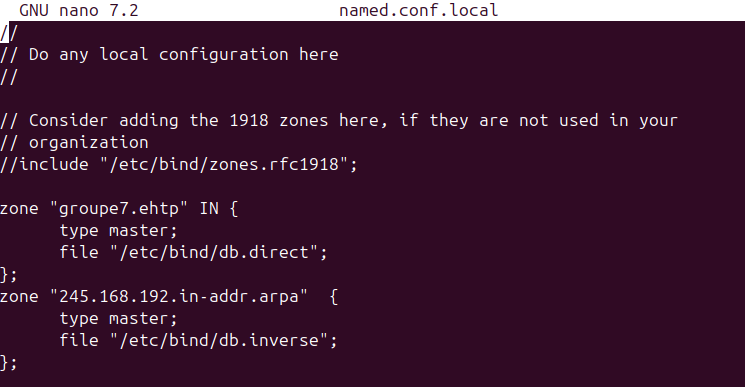
\includegraphics[width=0.7\textwidth]{DNS/named-conf-local.png}
		\caption{Configuration de \texttt{named.conf.local}}
		\label{fig:ridal}
	\end{figure}

	Pour vérifier s’il n’y a pas d’erreurs dans notre fichier \texttt{named.conf}, nous utilisons la commande suivante :
	\begin{lstlisting}[language=bash]
	named-checkconf
	\end{lstlisting}

	Ensuite, pour vérifier les fichiers \texttt{db.direct} et \texttt{db.inverse}, nous exécutons les commandes suivantes :
	
	\begin{lstlisting}[language=bash]
	sudo named-checkzone groupe7.ehtp /etc/bind/db.direct
	\end{lstlisting}
	
	\begin{figure}[h]
		\centering
		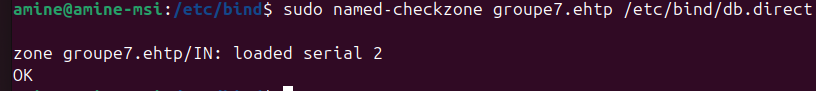
\includegraphics[width=0.7\textwidth]{DNS/checkzone_direct.png}
		\caption{Vérification de \texttt{db.direct}}
		\label{fig:ridal}
	\end{figure}

	\begin{lstlisting}[language=bash]
	sudo named-checkzone 245.168.192.in-addr.arpa /etc/bind/db.inverse
	\end{lstlisting}

	\begin{figure}[h]
		\centering
		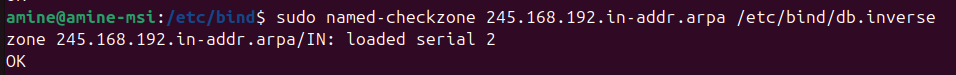
\includegraphics[width=0.7\textwidth]{DNS/checkzone_inverse.png}
		\caption{Vérification de \texttt{db.inverse}}
		\label{fig:ridal}
	\end{figure}

	Pour redémarrer le service BIND9, nous utilisons la commande suivante :
	
	\begin{lstlisting}[language=bash]
	sudo systemctl restart bind9
	\end{lstlisting}

	Enfin, pour tester la configuration DNS, nous ajoutons l’adresse IP du serveur DNS à une autre machine et exécutons la commande suivante :
	
	\begin{lstlisting}[language=bash]
	nslookup
	\end{lstlisting}
	
	\begin{figure}[h]
		\centering
		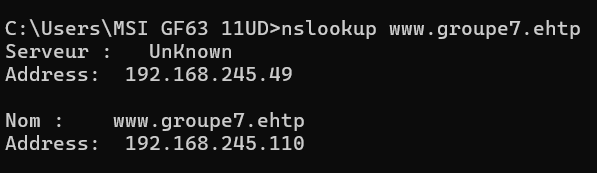
\includegraphics[width=0.7\textwidth]{DNS/test1.png}
		\caption{Vérification avec \texttt{nslookup}}
		\label{fig:ridal}
	\end{figure}

	Et voici le résultat de la commande avec l’adresse IP du serveur DNS :
	
	\begin{figure}[h]
		\centering
		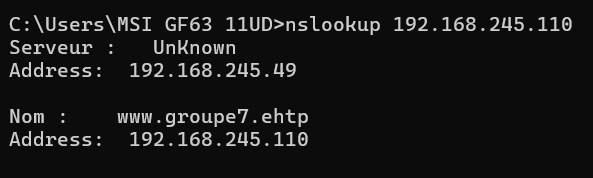
\includegraphics[width=0.7\textwidth]{DNS/test2.png}
		\caption{Résultat de la vérification}
		\label{fig:ridal}
	\end{figure}
	\newpage

	La configuration du serveur DNS est maintenant terminée avec succès.
	
	
	
		\newpage
	
		\newpage
\section{Configuration d'un Serveur HTTPS}

Le nom d'hôte du serveur : \texttt{groupe7.ehtp}  
Et son adresse IP : \texttt{192.168.245.49}.

Apache et OpenSSH sont des composants fondamentaux dans la mise en place d'un serveur web sécurisé et fonctionnel. Apache est un logiciel de serveur Web largement utilisé, réputé pour sa fiabilité et sa polyvalence dans la diffusion de contenu Web. Configurer Apache pour prendre en charge HTTPS implique d'activer le protocole SSL/TLS, qui crypte les données transmises entre le serveur et le client, garantissant ainsi une communication sécurisée. Cette sécurité est cruciale pour la transmission de données sensibles, telles que les identifiants de connexion, les informations financières et les détails personnels, faisant du HTTPS un protocole essentiel pour protéger la confidentialité des utilisateurs et l'intégrité des données.

D'autre part, OpenSSL, une implémentation robuste du protocole SSH (Secure Shell), offre un accès à distance sécurisé et facilite les transferts de fichiers sécurisés entre les systèmes. L'intégration d'OpenSSL dans l'environnement du serveur améliore la sécurité en permettant un accès à distance crypté pour l'administration du serveur et les transferts de fichiers sécurisés. Ensemble, Apache avec HTTPS et OpenSSH fournissent un environnement fortifié, garantissant la confidentialité et l'intégrité des communications Web tout en permettant une gestion à distance sécurisée du serveur.

\subsection*{1. Installer Apache}
Ouvrez un terminal et exécutez les commandes suivantes pour installer Apache sur votre serveur Ubuntu :

\begin{lstlisting}[language=bash]
sudo apt update
sudo apt install apache2
\end{lstlisting}

\subsection*{2. Vérifier le statut du service Apache}
Une fois Apache installé, vous pouvez vérifier que le service fonctionne correctement avec la commande suivante :

\begin{lstlisting}[language=bash]
sudo systemctl status apache2
\end{lstlisting}

Nous devons d’abord installer à la fois Apache et OpenSSL en exécutant la commande suivante :
\begin{lstlisting}[language=bash]
sudo apt-get install openssl apache2
\end{lstlisting}

La commande \texttt{a2enmod ssl} est utilisée dans le serveur HTTP Apache sur les systèmes basés sur Debian (tels que Ubuntu) pour activer le module SSL (Secure Sockets Layer) pour Apache. Après avoir exécuté cette commande, redémarrez le service Apache2 avec la commande suivante :

\begin{lstlisting}[language=bash]
sudo systemctl restart apache2
\end{lstlisting}

\subsection*{3. Créer un certificat SSL auto-signé}
Un certificat SSL auto-signé est un certificat numérique généré et signé par l'entité qu'il identifie, plutôt que par une autorité de certification (CA) tierce de confiance. Voici la commande pour générer un certificat SSL auto-signé :

\begin{lstlisting}[language=bash]
sudo openssl req -x509 -nodes -days 365 -newkey rsa:2048 -keyout /etc/ssl/private/private.key -out /etc/ssl/certs/certificate.crt
\end{lstlisting}

Lors de l'exécution de cette commande, vous devrez répondre aux invites.

Après avoir exécuté la commande, nous obtenons la clé générée dans le fichier spécifié.

\begin{figure}[h]
	\centering
	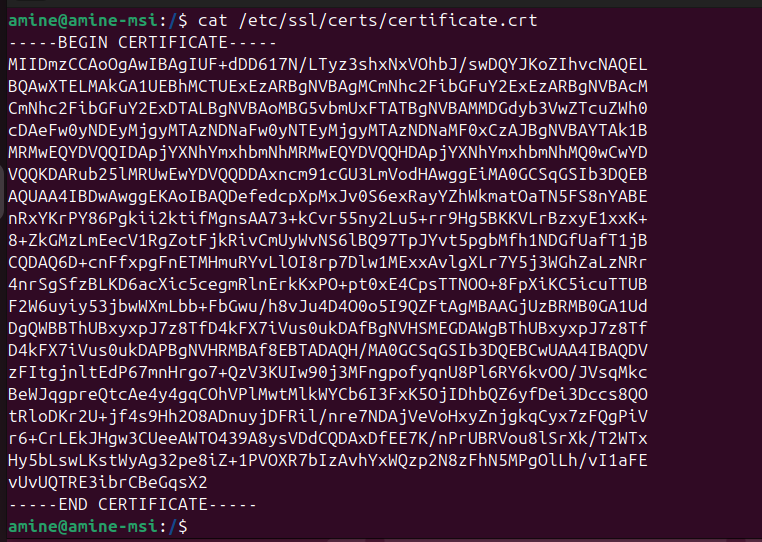
\includegraphics[width=0.7\textwidth]{HTTPS/certifcate.png}
	\caption{Certificat SSL auto-signé généré}
	\label{fig:certificate}
\end{figure}

\subsection*{4. Créer un fichier VirtualHost}
Créons maintenant notre fichier \texttt{VirtualHost}. Le fichier est à créer dans le dossier : \texttt{/etc/apache2/sites-available/}. Puisque Apache est livré avec un fichier VirtualHost par défaut, utilisons-le comme base. Nous copions le fichier \texttt{000-default.conf} vers \texttt{groupe7.conf} :

\begin{lstlisting}[language=bash]
sudo cp 000-default.conf groupe7.conf
\end{lstlisting}

Le fichier \texttt{groupe7.conf} devrait ressembler à ceci :
		\newpage

\begin{figure}[h]
	\centering
	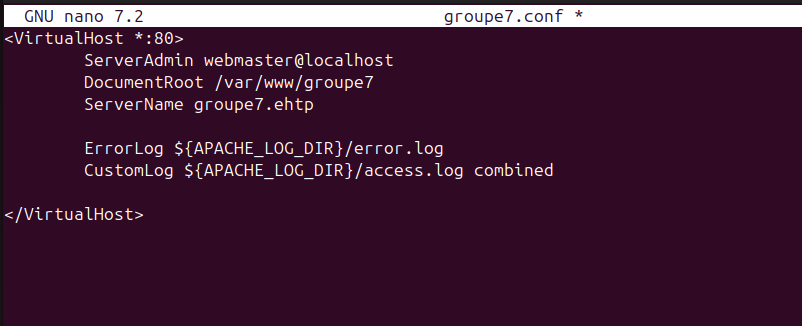
\includegraphics[width=0.7\textwidth]{HTTPS/groupe7-conf.png}
	\caption{Fichier \texttt{groupe7.conf}}
	\label{fig:groupe7conf}
\end{figure}

Après avoir configuré notre site Web, nous devons activer le fichier de configuration des hôtes virtuels pour l'activer. Nous faisons cela en exécutant la commande suivante dans le répertoire du fichier de configuration :

\begin{lstlisting}[language=bash]
sudo a2ensite groupe7.conf
\end{lstlisting}

\subsection*{5. Activer SSH sur Apache}
Maintenant que nous avons créé notre site, nous allons essayer d'activer SSH sur Apache. Créons le fichier \texttt{groupe7-ssl.conf} et ajoutons la configuration suivante :

\begin{figure}[h]
	\centering
	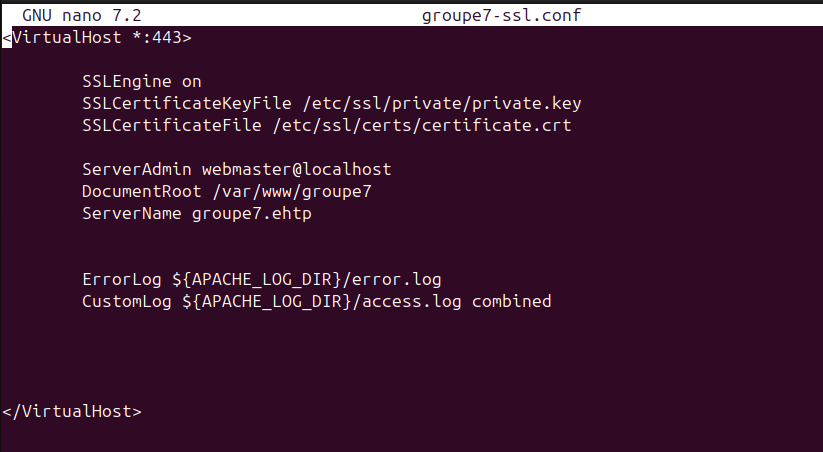
\includegraphics[width=0.7\textwidth]{HTTPS/groupe7-ssl-conf.png}
	\caption{Configuration de \texttt{groupe7-ssl.conf}}
	\label{fig:groupe7sslconf}
\end{figure}

Ensuite, nous devons ajouter \texttt{192.168.245.49 groupe7.ehtp} dans le fichier \texttt{/etc/hosts}.
\newpage

\begin{figure}[h]
	\centering
	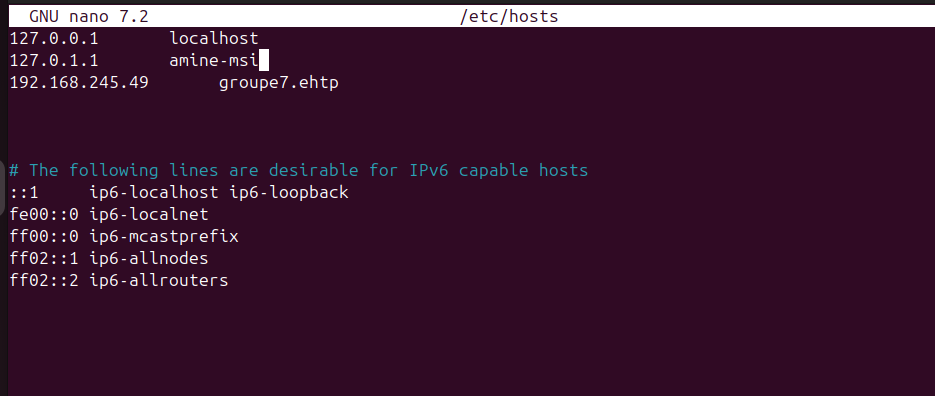
\includegraphics[width=0.7\textwidth]{HTTPS/host.png}
	\caption{Modification du fichier \texttt{/etc/hosts}}
	\label{fig:hosts}
\end{figure}

\subsection*{6. Créer le fichier index.html}
Ensuite, nous allons créer un fichier \texttt{index.html} dans le chemin \texttt{/var/www/groupe7/} :		

\begin{figure}[h]
	\centering
	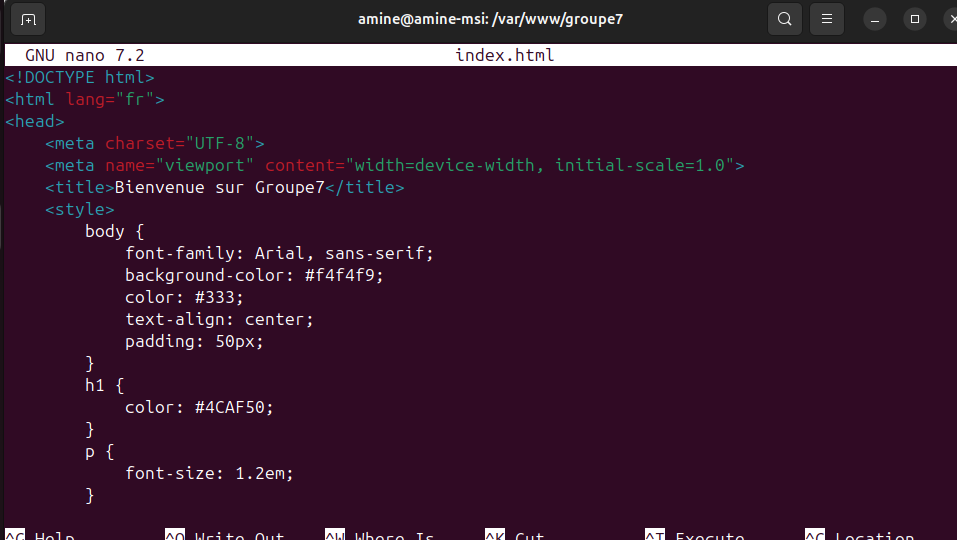
\includegraphics[width=0.7\textwidth]{HTTPS/index.png}
	\caption{Contenu du fichier \texttt{index.html}}
	\label{fig:index}
\end{figure}

\subsection*{7. Activer la version SSL de votre site}
Après cela, nous devons activer la version SSL de notre site. Nous pouvons exécuter cette commande pour activer le site :

\begin{lstlisting}[language=bash]
sudo a2ensite groupe7-ssl.conf
\end{lstlisting}

Nous pouvons vérifier la configuration Apache2 avec la commande suivante :

\begin{lstlisting}[language=bash]
sudo apache2ctl -t
\end{lstlisting}

S'il y avait des erreurs ou des fautes, elles apparaîtraient. Une fois aucune erreur, nous redémarrons le service Apache2 :

\begin{lstlisting}[language=bash]
sudo systemctl restart apache2
\end{lstlisting}

\subsection*{8. Vérification du statut d'Apache}
Une fois Apache redémarré, nous vérifions le statut avec la commande suivante :

\begin{lstlisting}[language=bash]
sudo systemctl status apache2
\end{lstlisting}

Voici le résultat affiché lorsque le serveur est actif :

\begin{figure}[h]
	\centering
	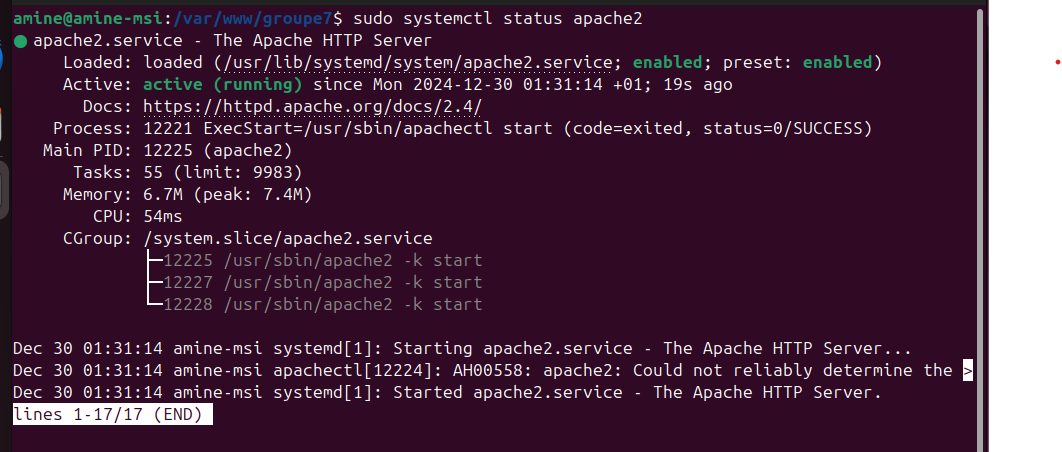
\includegraphics[width=0.7\textwidth]{HTTPS/status.png}
	\caption{Vérification du statut du service Apache2}
	\label{fig:status}
\end{figure}

\subsection*{9. Vérification du site}
Enfin, voici à quoi ressemble notre site après l'activation :

\begin{figure}[h]
	\centering
	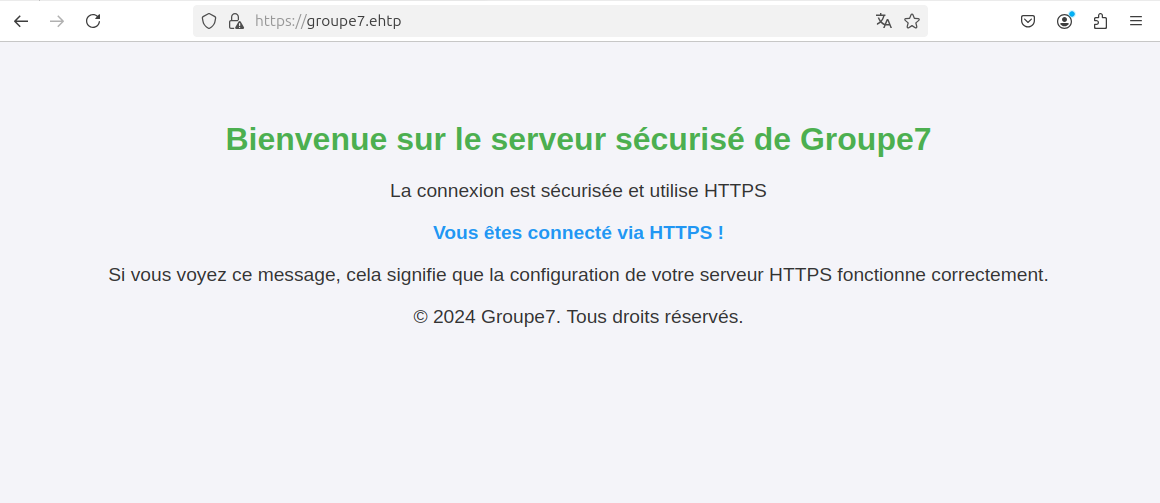
\includegraphics[width=0.7\textwidth]{HTTPS/test1.png}
	\caption{Vérification du site HTTPS}
	\label{fig:test1}
\end{figure}

\newpage







\section{Installation et Configuration de FTP}

\subsection*{1. Installation de \texttt{vsftpd}}
Pour installer \texttt{vsftpd}, commencez par mettre \`a jour la liste des paquets disponibles, puis ex\'ecutez les commandes suivantes :

\begin{lstlisting}[language=bash]
sudo apt update
sudo apt install vsftpd
\end{lstlisting}

\subsection*{2. V\'erification de l'\'etat du service FTP}
Apr\`es l'installation, assurez-vous que le service \texttt{vsftpd} est actif et en cours d'ex\'ecution en utilisant la commande suivante :

\begin{lstlisting}[language=bash]
sudo systemctl status vsftpd
\end{lstlisting}

\begin{figure}[h]
	\centering
	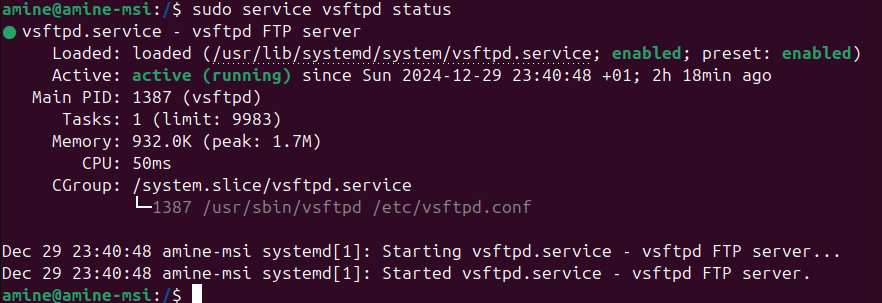
\includegraphics[width=0.7\textwidth]{FTP/status.png}
	\caption{\'Etat du service \texttt{vsftpd}}
	\label{fig:status}
\end{figure}

\subsection*{3. Configuration du serveur FTP}
Le fichier de configuration principal de \texttt{vsftpd} se trouve \`a l'emplacement suivant :

\begin{lstlisting}[language=bash]
/etc/vsftpd.conf
\end{lstlisting}

Pour le modifier, utilisez la commande suivante :

\begin{lstlisting}[language=bash]
sudo nano /etc/vsftpd.conf
\end{lstlisting} 
\newpage

\begin{figure}[h]
	\centering
	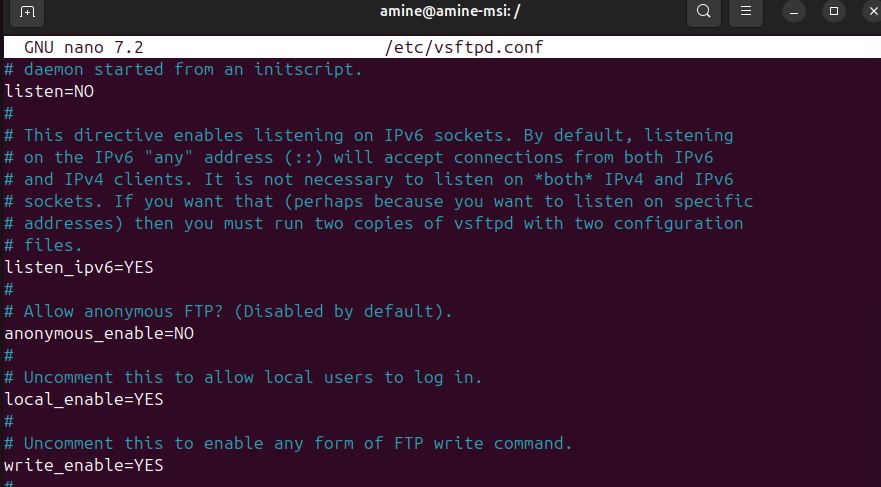
\includegraphics[width=0.7\textwidth]{FTP/vsftp-conf1.png}
	\caption{Exemple de configuration de \texttt{vsftpd} (partie 1)}
	\label{fig:conf1}
\end{figure}

\begin{figure}[h]
	\centering
	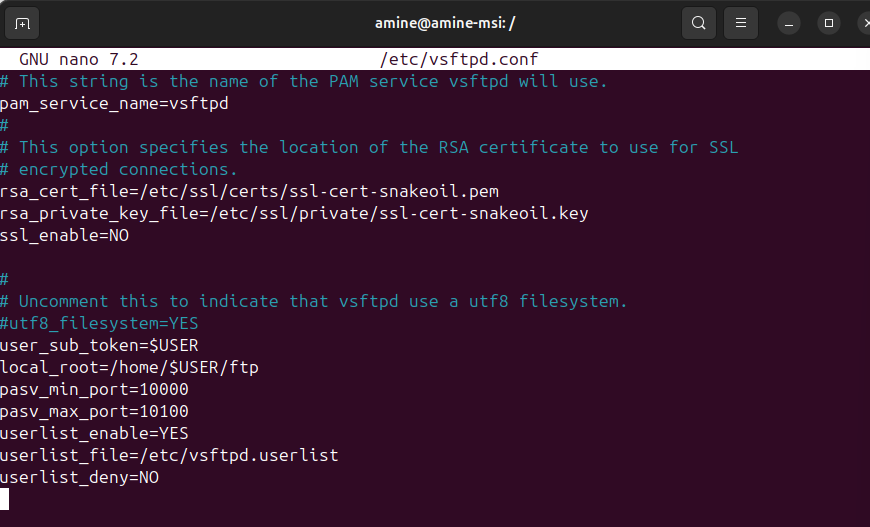
\includegraphics[width=0.7\textwidth]{FTP/vsftp-conf2.png}
	\caption{Exemple de configuration de \texttt{vsftpd} (partie 2)}
	\label{fig:conf2}
\end{figure}

\subsection*{4. Configuration du pare-feu}
Pour permettre au serveur FTP de fonctionner correctement, ouvrez les ports requis en utilisant la commande suivante :

\begin{lstlisting}[language=bash]
sudo ufw allow from any to any port 20,21,10000,10100 proto tcp
\end{lstlisting}

\begin{figure}[h]
	\centering
	
\includegraphics[width=0.7\textwidth]{FTP/proto.png}
	\caption{Configuration du pare-feu}
	\label{fig:firewall}
\end{figure}

\subsection*{5. Cr\'eation d'un utilisateur FTP}
Pour ajouter un utilisateur ayant acc\`es au serveur FTP, ex\'ecutez la commande suivante :

\begin{lstlisting}[language=bash]
sudo adduser nourddine
\end{lstlisting}

Ensuite, cr\'eez un r\'epertoire FTP pour cet utilisateur :

\begin{lstlisting}[language=bash]
sudo mkdir /home/nourddine/ftp
\end{lstlisting}

Affectez les permissions appropri\'ees au r\'epertoire :

\begin{lstlisting}[language=bash]
sudo chown nobody:nogroup /home/nourddine/ftp
\end{lstlisting}

Enfin, ajoutez un sous-r\'epertoire pour les t\'el\'echargements :

\begin{lstlisting}[language=bash]
sudo mkdir /home/nourddine/ftp/upload
\end{lstlisting}

\begin{figure}[h]
	\centering
	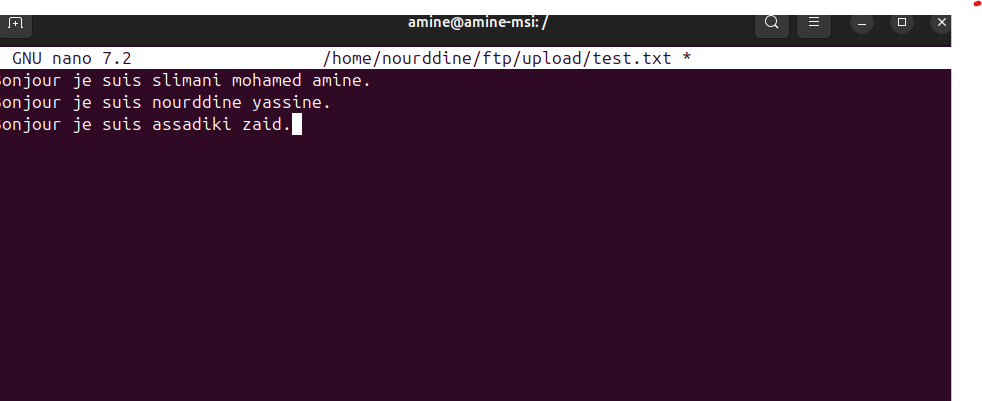
\includegraphics[width=0.7\textwidth]{FTP/fichier.png}
	\caption{Test du r\'epertoire FTP}
	\label{fig:ftp-test}
\end{figure}

\subsection*{6. Ajout de l'utilisateur \`a la liste FTP}
Modifiez le fichier \texttt{/etc/vsftpd.userlist} pour y ajouter le nouvel utilisateur :

\begin{lstlisting}[language=bash]
sudo nano /etc/vsftpd.userlist
\end{lstlisting}

\begin{figure}[h]
	\centering
	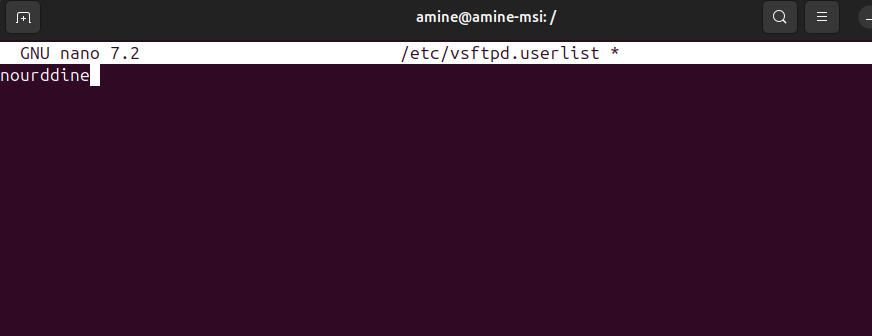
\includegraphics[width=0.7\textwidth]{FTP/user_list.png}
	\caption{Ajout de l'utilisateur \`a la liste \texttt{vsftpd.userlist}}
	\label{fig:userlist}
\end{figure}

\subsection*{7. Test de la connexion FTP}
Vous pouvez tester la connexion au serveur FTP en utilisant deux m\'ethodes :

\paragraph{M\'ethode 1 : Via FileZilla}
Utilisez FileZilla pour vous connecter au serveur en fournissant les informations de connexion.

\begin{figure}[h]
	\centering
	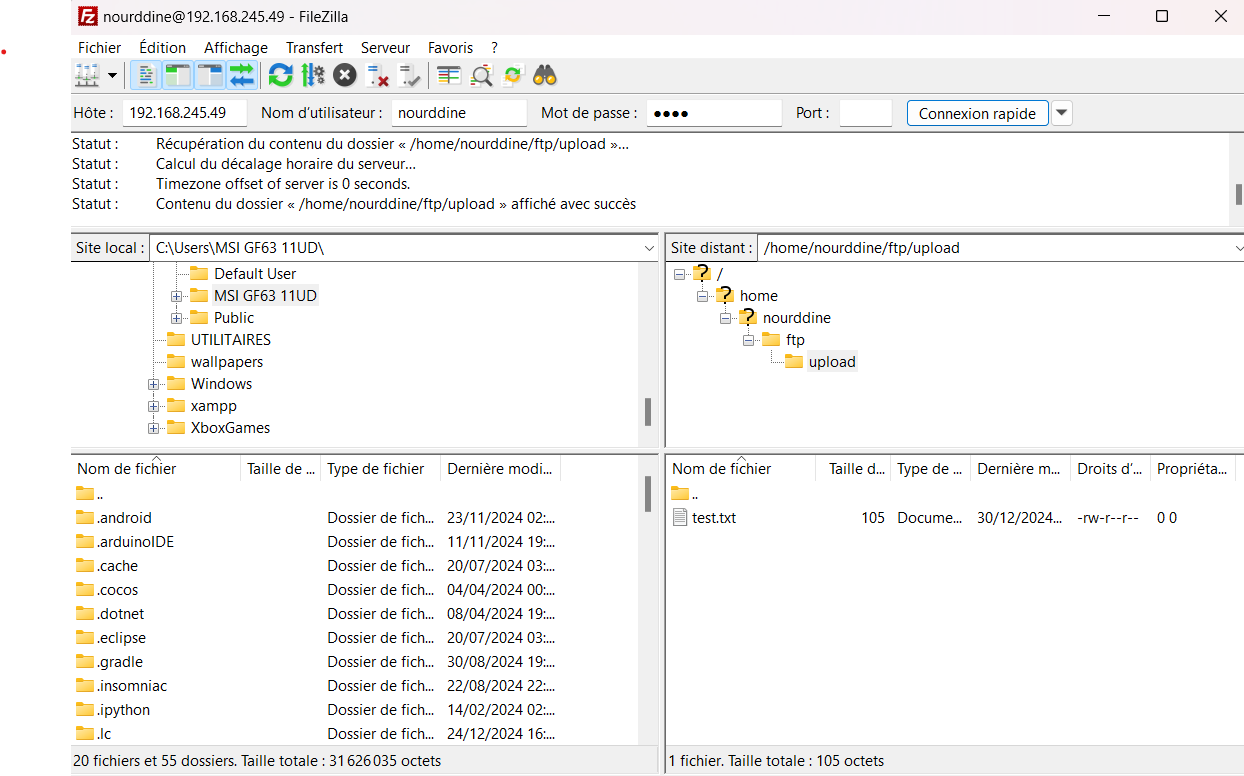
\includegraphics[width=0.7\textwidth]{FTP/fire.png}
	\caption{Connexion via FileZilla}
	\label{fig:filezilla}
\end{figure}

\paragraph{M\'ethode 2 : Via la ligne de commande}
Utilisez la commande FTP dans l'invite de commandes de Windows :
\newpage
\begin{figure}[h]
	\centering
	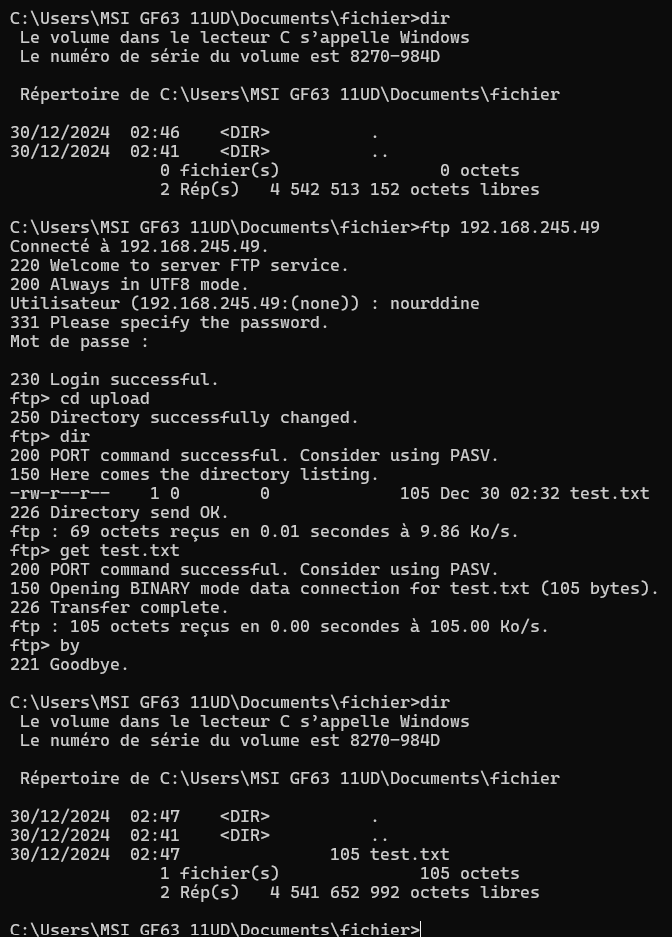
\includegraphics[width=0.7\textwidth]{FTP/test.png}
	\caption{Connexion via l'invite de commande Windows}
	\label{fig:cmd}
\end{figure}



\newpage



\section{Installation et Configuration du Serveur de Messagerie (SMTP/IMAP)}

\subsection*{1. Installer et Configurer Postfix}
Tout d'abord, installez le serveur de messagerie \texttt{Postfix} en exécutant la commande suivante :

\begin{lstlisting}[language=bash]
sudo apt-get install postfix
\end{lstlisting}

Ensuite, reconfigurez \texttt{Postfix} en utilisant la commande suivante pour définir les options de configuration, telles que la liste des domaines gérés par le serveur (par exemple, \texttt{groupe7.ehtp}) :

\begin{lstlisting}[language=bash]
sudo dpkg-reconfigure postfix
\end{lstlisting}

Après la configuration, redémarrez le service \texttt{Postfix} :

\begin{lstlisting}[language=bash]
sudo systemctl restart postfix
\end{lstlisting}

Vérifiez que le serveur écoute sur le port 25 en exécutant la commande suivante :

\begin{lstlisting}[language=bash]
sudo netstat -apn --inet
\end{lstlisting}

\begin{figure}[h]
	\centering
	
\includegraphics[width=0.7\textwidth]{SMTP/port.png}
	\caption{le serveur écoute sur le port 25 }
	\label{fig:cmd}
\end{figure}

\subsection*{2. Installer et Configurer Dovecot IMAP}
Installez le serveur \texttt{IMAP} en exécutant la commande suivante pour installer \texttt{Dovecot IMAP} :

\begin{lstlisting}[language=bash]
sudo apt-get install dovecot-imapd
\end{lstlisting}

Vérifiez ensuite que le serveur écoute sur le port IMAP (port 143) avec la commande suivante :

\begin{lstlisting}[language=bash]
sudo netstat -apn --inet
\end{lstlisting}

\begin{figure}[h]
	\centering
	
\includegraphics[width=0.7\textwidth]{SMTP/143.png}
	\caption{le serveur écoute sur le port 143}
	\label{fig:cmd}
\end{figure}

\subsection*{3. Créer des Utilisateurs et Répertoires}
Créez deux utilisateurs \texttt{user1} et \texttt{user2} et leurs répertoires respectifs avec les commandes suivantes :

\begin{lstlisting}[language=bash]
sudo useradd -m -d /home/user1 user1
sudo useradd -m -d /home/user2 user2
\end{lstlisting}

\subsection*{4. Installer le Client de Messagerie Thunderbird}
Installez le client de messagerie \texttt{Thunderbird} en exécutant la commande suivante :

\begin{lstlisting}[language=bash]
sudo apt-get install thunderbird
\end{lstlisting}

Après l'installation, définissez le mot de passe de \texttt{user1} avec la commande suivante :

\begin{lstlisting}[language=bash]
sudo passwd user1
\end{lstlisting}

Lancez ensuite \texttt{Thunderbird}, créez un nouvel utilisateur et configurez-le pour tester la réception et l'envoi d'emails.

\begin{figure}[h]
	\centering
	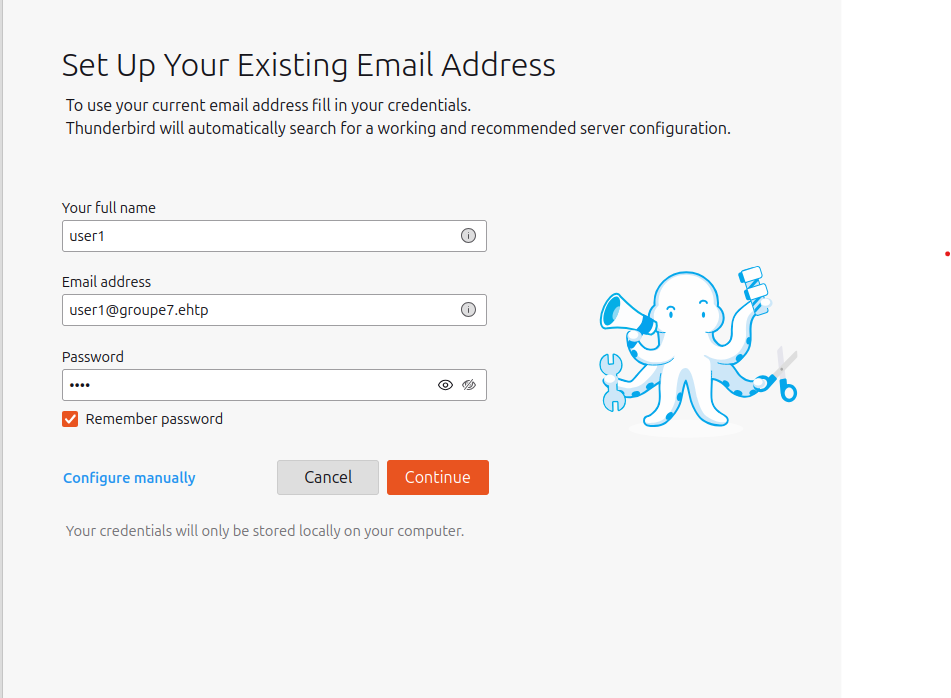
\includegraphics[width=0.7\textwidth]{SMTP/user1_email.png}
	\caption{Configuration du compte utilisateur \texttt{user1} dans Thunderbird}
	\label{fig:cmd}
\end{figure}

\subsection*{5. Tester l'Envoi et la Réception des Emails}
Avant le test, voici le tableau de bord de \texttt{Thunderbird} avec le compte configuré :
\newpage
\begin{figure}[h]
	\centering
	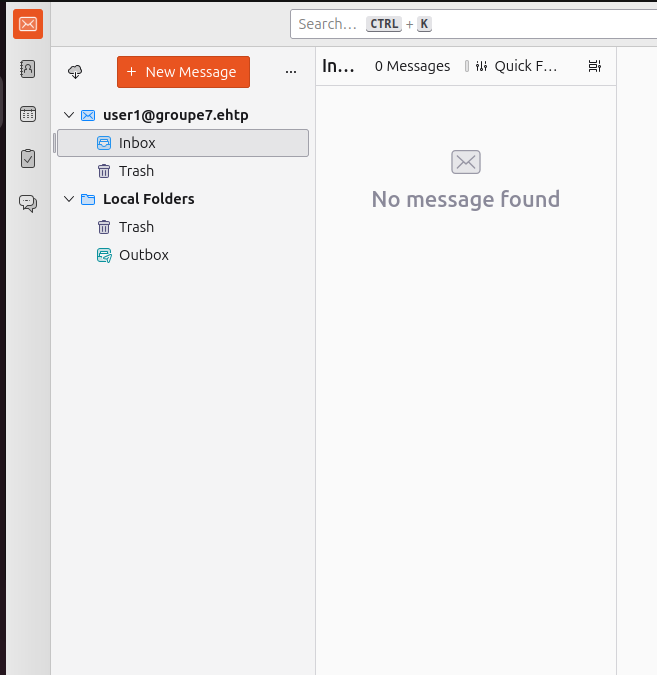
\includegraphics[width=0.7\textwidth]{SMTP/da.png}
	\caption{Tableau de bord de Thunderbird avant le test}
	\label{fig:cmd}
\end{figure}

Pour tester l'envoi d'un email, connectez-vous au serveur SMTP en utilisant la commande suivante dans l'invite de commande :

\begin{lstlisting}[language=bash]
telnet 127.0.0.1 25
\end{lstlisting}

Ensuite, envoyez un email en utilisant les commandes SMTP et vérifiez que l'email est bien reçu dans la boîte de réception de \texttt{Thunderbird} :
\newpage

\begin{figure}[h]
	\centering
	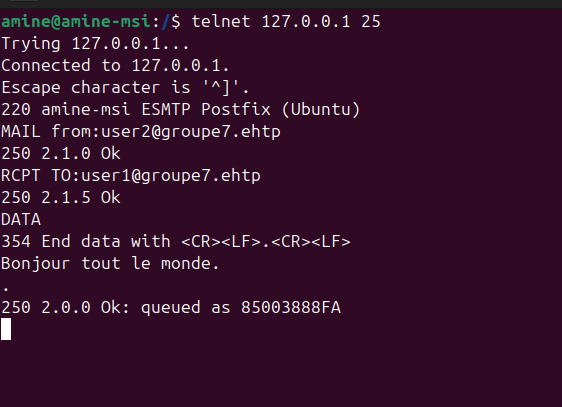
\includegraphics[width=0.7\textwidth]{SMTP/toto.png}
	\caption{Envoi d'un email via l'invite de commande}
	\label{fig:cmd}
\end{figure}

Enfin, voici la réception de l'email dans la boîte de réception de \texttt{Thunderbird} :

\begin{figure}[h]
	\centering
	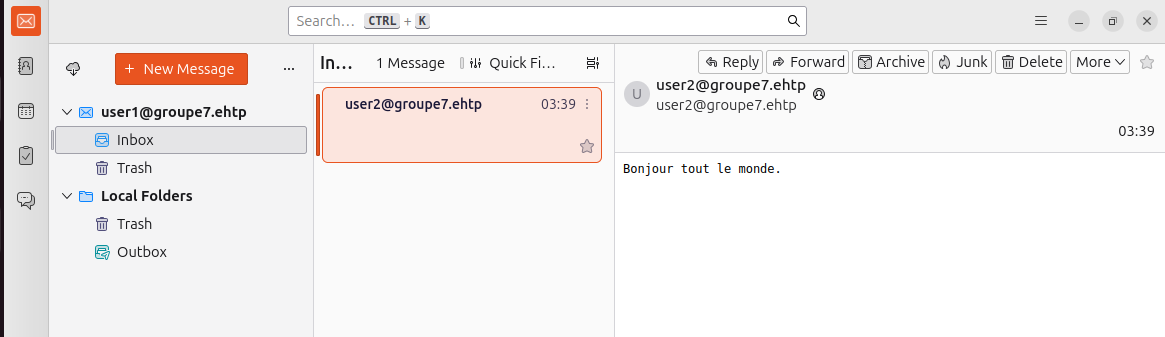
\includegraphics[width=0.7\textwidth]{SMTP/rcpt.png}
	\caption{Réception de l'email dans Thunderbird}
	\label{fig:cmd}
\end{figure}
	\newpage
\section{Installation et Configuration du Serveur LDAP}

Dans le cadre de notre projet réseau, nous avons implémenté OpenLDAP comme serveur d'annuaire centralisé. Le serveur, identifié par le nom d'hôte \texttt{ldap.groupe7.ehtp} et l'adresse IP \texttt{192.168.245.29}, joue un rôle crucial en stockant et organisant les informations relatives aux utilisateurs, groupes, et ressources réseau. Cette configuration vise à garantir une gestion efficace et sécurisée des données.

\subsection*{Installation d'OpenLDAP}
nous procédons à l'installation d'OpenLDAP :
\begin{lstlisting}[language=bash]
sudo apt install slapd ldap-utils -y
\end{lstlisting}

Une fois l'installation terminée, la commande suivante permet de vérifier la configuration initiale :
\begin{lstlisting}[language=bash]
sudo slapcat
\end{lstlisting}

\begin{figure}[h]
	\centering
	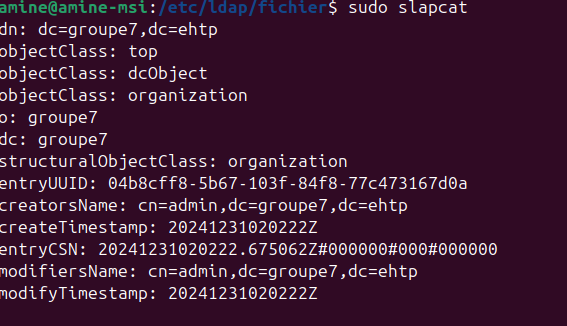
\includegraphics[width=0.7\textwidth]{LDAP/slapcat1.png}
	\caption{Résultat de la commande \texttt{slapcat}}
	\label{fig:slapcat1}
\end{figure}

\subsection*{Configuration de l'Annuaire}
Nous créons un répertoire dédié pour stocker les fichiers de configuration :
\begin{lstlisting}[language=bash]
sudo mkdir /etc/ldap/fichier
\end{lstlisting}

Dans ce répertoire, un fichier \texttt{utilisateurs\_et\_groupes.ldif} est créé pour définir les utilisateurs et groupes. Voici un exemple du contenu :

\begin{figure}[h]
	\centering
	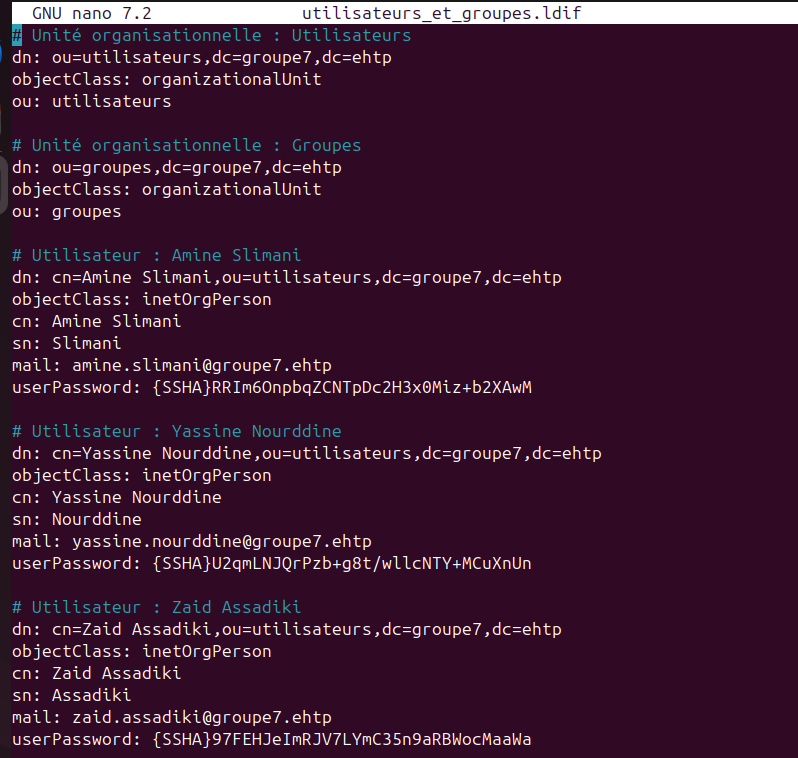
\includegraphics[width=0.7\textwidth]{LDAP/ut1.png}
	\caption{Exemple de contenu du fichier \texttt{utilisateurs\_et\_groupes.ldif}}
	\label{fig:ut1}
\end{figure}

\subsection*{Gestion des Mots de Passe}
Les mots de passe des utilisateurs sont hachés avec l’algorithme SSHA. Pour générer un mot de passe sécurisé, utilisez :
\begin{lstlisting}[language=bash]
slappasswd
\end{lstlisting}

\begin{figure}[h]
	\centering
	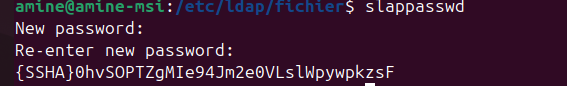
\includegraphics[width=0.7\textwidth]{LDAP/slap.png}
	\caption{Génération de mots de passe avec \texttt{slappasswd}}
	\label{fig:slap}
\end{figure}

\subsection*{Ajout des Données dans l'Annuaire}
Pour intégrer les données définies dans \texttt{utilisateurs\_et\_groupes.ldif} dans l'annuaire :
\begin{lstlisting}[language=bash]
ldapadd -x -D "cn=admin,dc=groupe7,dc=ehtp" -w admin_password -f utilisateurs_et_groupes.ldif
\end{lstlisting}

\begin{figure}[h]
	\centering
	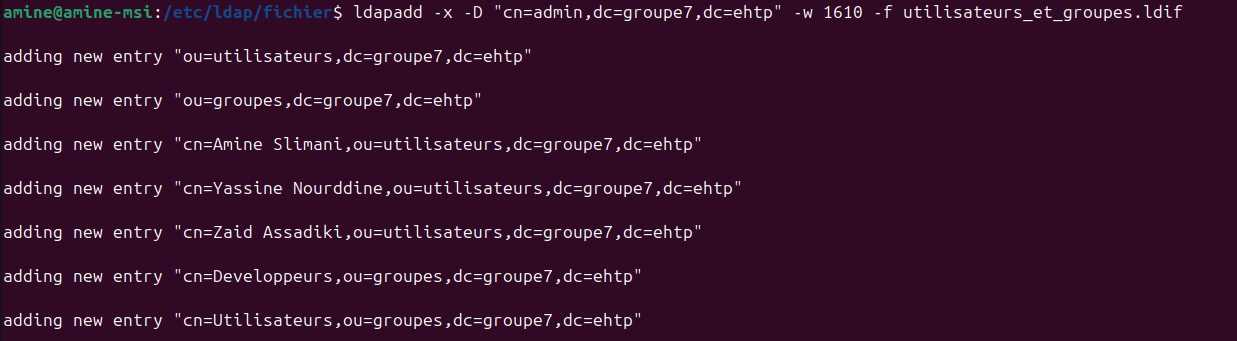
\includegraphics[width=0.7\textwidth]{LDAP/add.png}
	\caption{Ajout des données dans l'annuaire LDAP}
	\label{fig:add}
\end{figure}

La commande suivante permet de vérifier les données ajoutées :
\begin{lstlisting}[language=bash]
sudo slapcat
\end{lstlisting}

\begin{figure}[h]
	\centering
	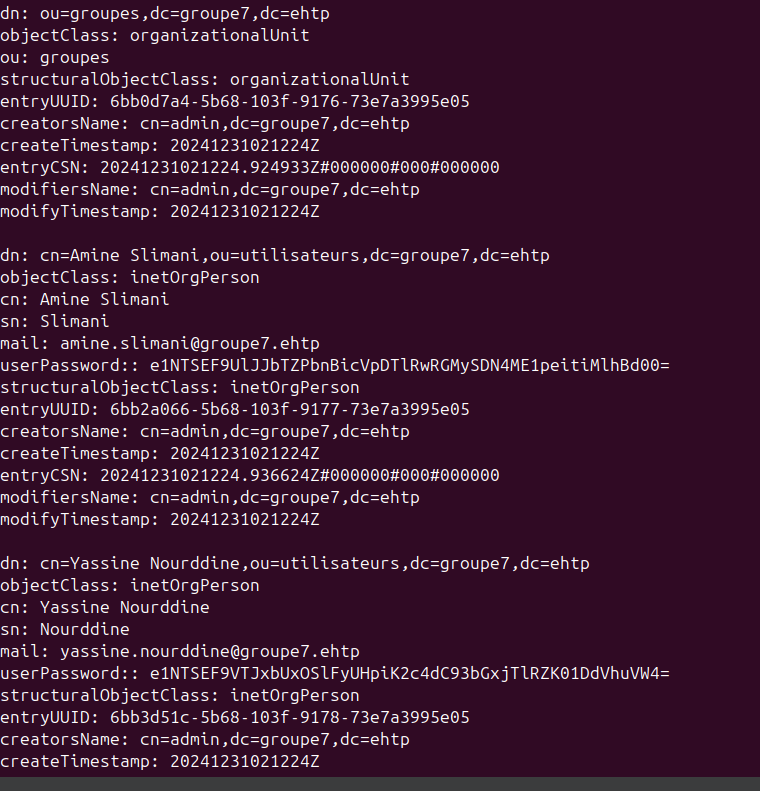
\includegraphics[width=0.7\textwidth]{LDAP/slapcat2.png}
	\caption{Vérification des utilisateurs dans l'annuaire LDAP}
	\label{fig:slapcat2}
\end{figure}

\subsection*{Installation et Configuration de l'Interface Web PHPLDAPADMIN}
PHPLDAPADMIN est un outil graphique qui simplifie la gestion du serveur LDAP. Pour l'installer :
\begin{lstlisting}[language=bash]
sudo apt-get install phpldapadmin
\end{lstlisting}

Configuration :
\begin{lstlisting}[language=bash]
sudo gedit /etc/phpldapadmin/config.php
\end{lstlisting}

Les paramètres suivants sont ajoutés au fichier :
\newpage
\begin{figure}[h]
	\centering
	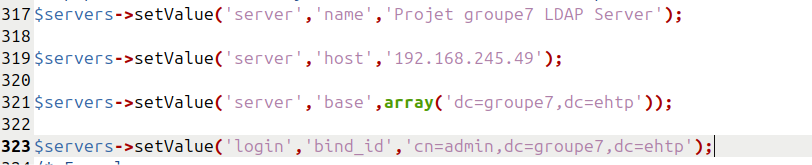
\includegraphics[width=0.7\textwidth]{LDAP/conf.png}
	\caption{Configuration du fichier \texttt{config.php}}
	\label{fig:conf}
\end{figure}

Pour accéder à l'interface, ouvrez un navigateur et saisissez :
\begin{figure}[h]
	\centering
	
\includegraphics[width=0.7\textwidth]{LDAP/t.png}
	\caption{Connexion à PHPLDAPADMIN via le navigateur}
	\label{fig:t}
\end{figure}

Le tableau de bord de l'interface Web ressemble à ceci :
\begin{figure}[h]
	\centering
	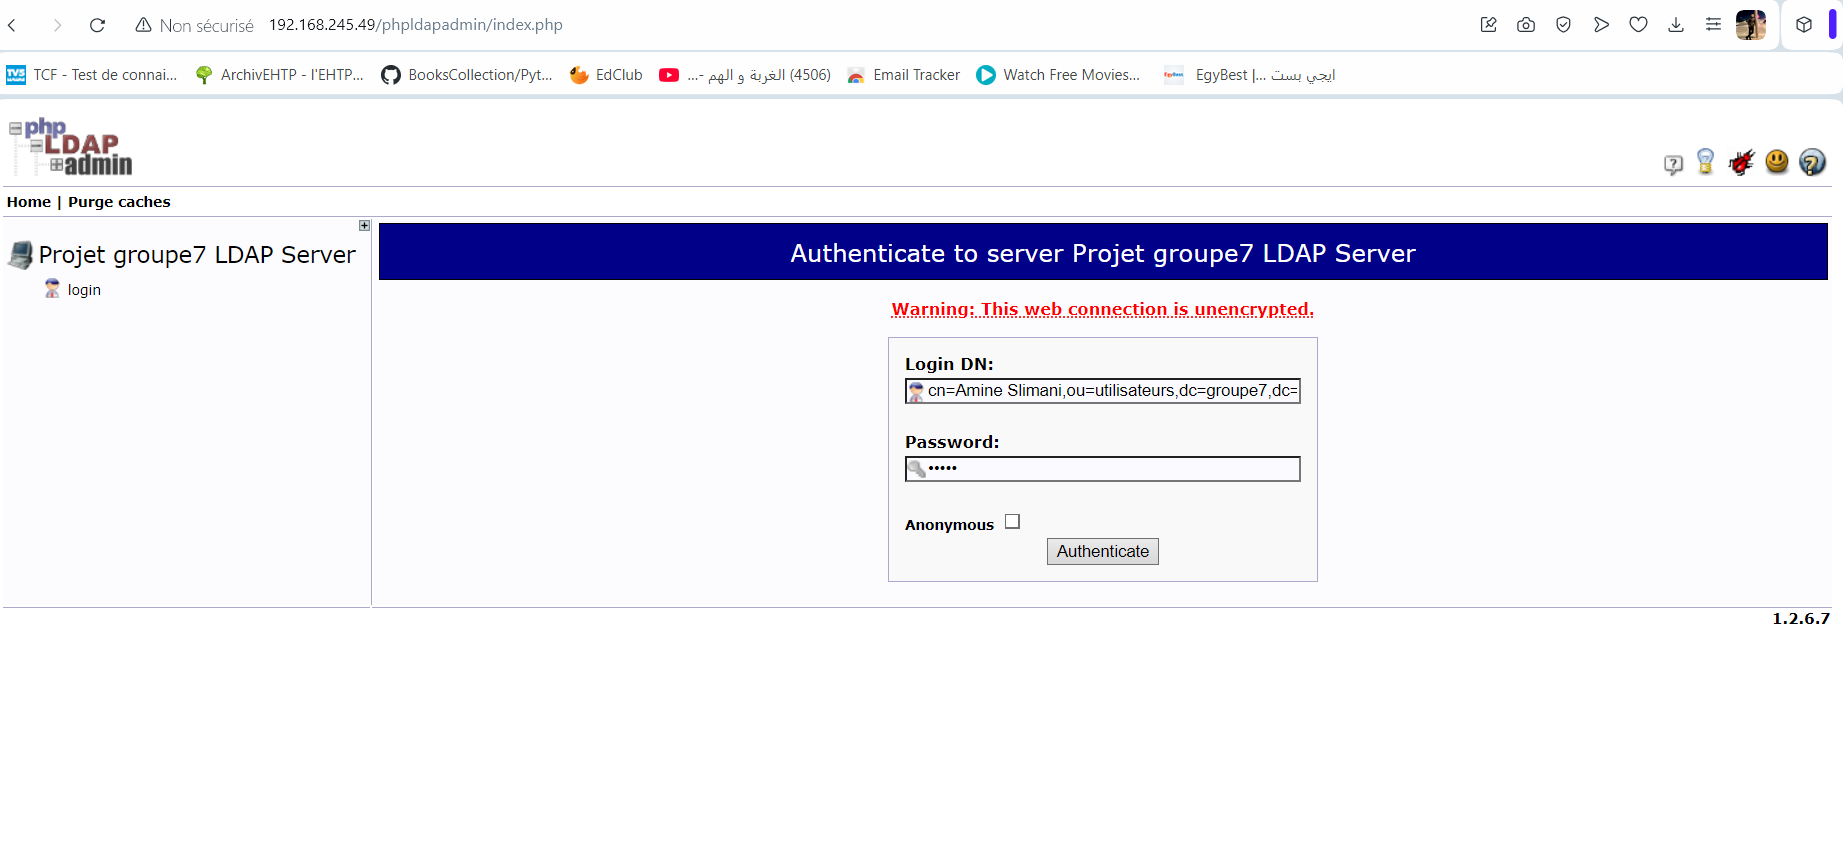
\includegraphics[width=0.7\textwidth]{LDAP/test1.png}
	\caption{Tableau de bord de PHPLDAPADMIN}
	\label{fig:test1}
\end{figure}

Après connexion, les utilisateurs et groupes peuvent être visualisés et gérés via cette interface conviviale.


\begin{figure}[h!]
	\centering
	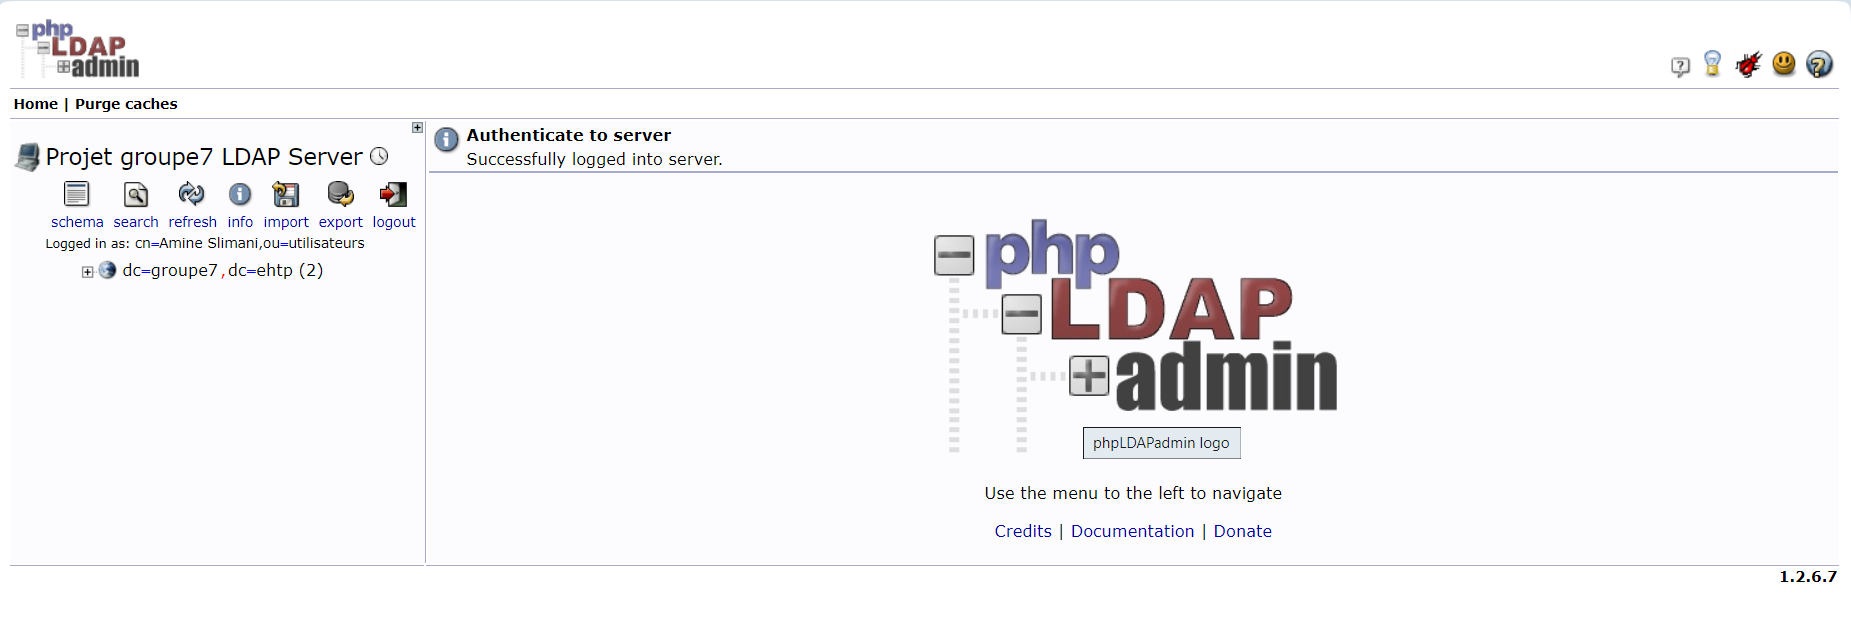
\includegraphics[width=0.7\textwidth]{LDAP/test2.png}
	\caption{Visualisation des utilisateurs et groupes dans PHPLDAPADMIN}
	\label{fig:test2}
\end{figure}

		\newpage
\section{Conclusion}

En conclusion, ce projet nous a permis de mettre en œuvre et de configurer des protocoles réseau essentiels tels que DNS, HTTPS, FTP, SMTP, IMAP, et LDAP, afin de garantir une infrastructure réseau fiable, performante et sécurisée. Ces configurations, bien que techniquement exigeantes, ont renforcé la connectivité et la protection des données tout en facilitant la gestion centralisée des utilisateurs et des ressources grâce à OpenLDAP.

Les défis rencontrés, notamment en matière de compatibilité, de sécurité, et de performances, ont été surmontés grâce à une méthodologie rigoureuse et une veille technologique continue. Ce travail nous a permis d'acquérir une meilleure compréhension des exigences et des bonnes pratiques liées à la gestion des réseaux modernes.

Ainsi, le projet pose les bases d’une infrastructure résiliente et évolutive, prête à répondre aux besoins actuels et futurs, tout en offrant un environnement sécurisé et performant pour les utilisateurs et les systèmes connectés.  






\end{document}
